\section{Loop}

\subsection{Allgemein}

Charles Loop hat 1987 einen Unterteilungsalgorithmus für Dreiecksnetze entwickelt.
Der Loop Algorithmus basiert auf quartischen Box Splines und approximiert die Kontrollpunkte.
An extraordinären Stellen mit Valence ungleich sechs erzeugt Loop \(C^1\) stetige Flächen,
im regulären Fall ansonsten \(C^2\).
\cite[S. 70f]{Zorin.subdivcourse} \cite[S. 56f]{Standford.24.07.2015}

\subsection{Unterteilungsregel}

Die Unterteilung erfolgt in drei Schritten.
\begin{enumerate}
\item Berechne für jede Kante einen edge point. Dieser wird auch als odd Vertex bezeichnet.
\item Berechne für jeden Vertex eine neue Position. Dieser wird auch als even Vertex bezeichnet.
\item Ersetze jede Dreieck durch vier neue Dreiecke.
\end{enumerate}

\begin{figure}
\centering
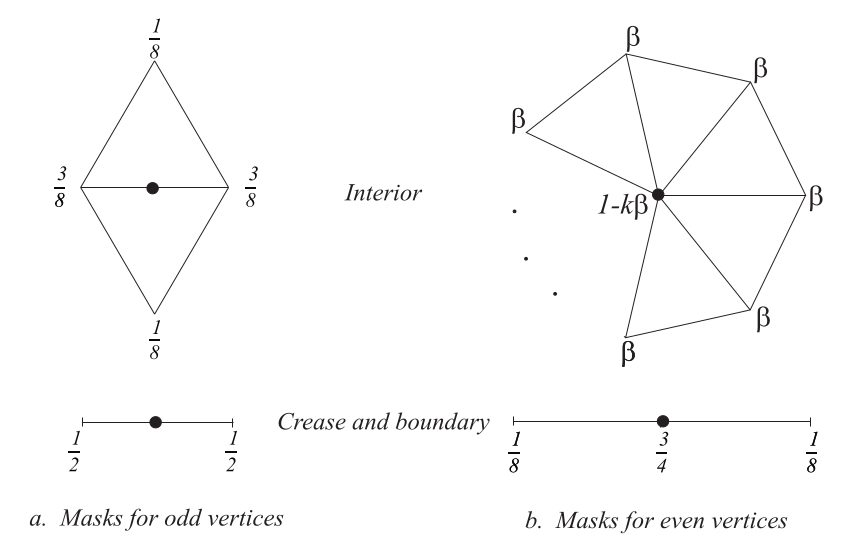
\includegraphics[width=1.0\textwidth]{content/media/sd_loop_mask.jpg}
\caption{Loop Maske \cite[S. 70f]{Zorin.subdivcourse}}
\label{fig:sd_loop_mask}
\end{figure}

\subsubsection*{Odd Vertex}

\subsubsection*{Even Vertex}

\subsubsection*{Face Split}


\begin{figure}
\centering
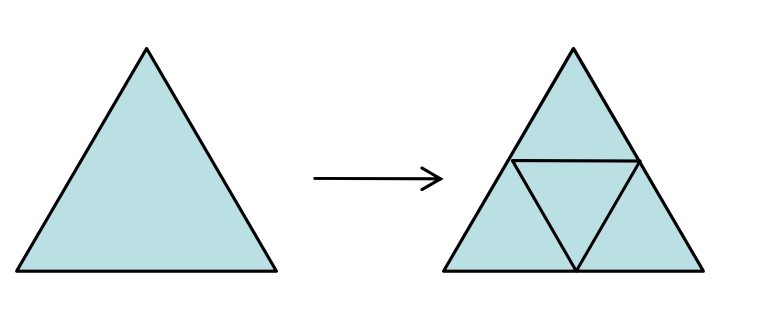
\includegraphics[width=0.3\textwidth]{content/media/sd_loop_split.png}
\caption{Loop face split \cite[S. 56f]{Standford.24.07.2015}}
\label{fig:sd_loop_split}
\end{figure}

\subsection{Boundary}

